\section{Fractional Differential Equations}

\subsection{Adams-Bashforth-Moulton Predictor-Corrector Algorithm}\label{sec:ABM}
The Adams-Bashforth-Moulton Predictor-Corrector method (ABM method), first proposed by Diethelm \textit{et al.} in \cite{diethelm2002predictor}, is a numerical algorithm to solve a fractional differential equation (FDE) in the form:

\begin{equation}\label{eq:frac_dif}
\begin{cases}
     \mathcal { D } _ { c } ^ { \alpha }y(t) = f(t,y)&\\ y(0)=y_0,\,\dots,y^{(\ceil{\alpha} - 1)}(0)= y_{(\ceil{\alpha} - 1)}\quad t\in[0,T]&
\end{cases}
\end{equation}

Applying the theorem \ref{theo:rightinverse} to \ref{eq:frac_dif} we get the following equation:
\begin{equation*}
    y(t)=\sum _{ k=0 }^{ m-1 }{ { y }_{ (k) }\frac { { x }^{ k } }{ k! }  } +\frac { 1 }{ \Gamma (\alpha ) } \int _{ 0 }^{ t }{ { (t-\lambda ) }^{ \alpha -1 }f(\lambda ,y(\lambda ))d\lambda  } 
\end{equation*}

Then, as explained in \cite{diethelm2002predictor}, the integral is approximated by quadrature theory. With this approximation, it is obtained that:

\begin{equation}
    \begin{aligned} y _ { h } \left( t _ { n + 1 } \right) = & \sum _ { k = 0 } ^ { [ \alpha ] - 1 } \frac { t _ { n + 1 } ^ { k } } { k ! } y _ { ( k ) } + \frac { h ^ { \alpha } } { \Gamma ( \alpha + 2 ) } f \left( t _ { n + 1 } , y _ { h } ^ { \mathrm { p } } \left( t _ { n + 1 } \right) \right) \\ & + \frac { h ^ { \alpha } } { \Gamma ( \alpha + 2 ) } \sum _ { j = 0 } ^ { n } a _ { j , n + 1 } f \left( t _ { j } , y _ { h } \left( t _ { j } \right) \right) \end{aligned}
\end{equation}

With:
\begin{equation*}
    a _ { j , n + 1 } = \left\{ \begin{array} { l l } { n ^ { \alpha + 1 } - ( n - \alpha ) ( n + 1 ) ^ { \alpha } , } & { \text { if } j = 0 } \\ { ( n - j + 2 ) ^ { \alpha + 1 } + ( n - j ) ^ { \alpha + 1 } - 2 ( n - j + 1 ) ^ { \alpha + 1 } , } & { \text { if } 1 \leq j \leq n } \\ { 1 , } & { \text { if } j = n + 1 } \end{array} \right.
\end{equation*}

And $y _ { h } ^ { \mathrm { p } } \left( t _ { n + 1 } \right)$ being a predicted value for the variable. To find this prediction, instead of approximating the integral by quadrature theory the product rectangle rule is used. Therefore, it is found that:

\begin{equation*}
    y _ { h } ^ { \mathrm { P } } \left( t _ { n + 1 } \right) = \sum _ { k = 0 } ^ { \lceil \alpha ] - 1 } \frac { t _ { n + 1 } ^ { k } } { k ! } y _ { ( k ) } + \frac { 1 } { \Gamma ( \alpha ) } \sum _ { j = 0 } ^ { n } b _ { j , n + 1 } f \left( t _ { j } , y _ { h } \left( t _ { j } \right) \right)
\end{equation*}

With:
\begin{equation*}
    b _ { j , n + 1 } = \frac { h ^ { \alpha } } { \alpha } \left( ( n + 1 - j ) ^ { \alpha } - ( n - j ) ^ { \alpha } \right)
\end{equation*}

There are some important aspects to notice about this method. First of all, for every iteration it needs every iteration prior because fractional derivatives have memory; but, this makes the algorithm to have a worst algorithmic complexity as the integer case (improvements for this will be discussed in chapter \ref{chap:modif}). Lastly, it is seen that a predicted value is necessary for calculating every iteration so, why don't use this predicted value instead as the real value instead that do not needs prediction before?; this is done because, adding a new iteration corrects some errors that the last prediction could have (this is similar at how RK4 works).

Some modifications for this algorithm can be seen at section \ref{sec:predABM}.

\subsubsection{Pseudo-Code}
\textbf{Input Variables}
\begin{equation*}
\begin{array}{ll}
f=&\text{real-valued function defined for right side of the differential equation.}\\
\alpha=&\text{the order of the fractional differential equation, real and positive number.}\\
y_0=&\text{array of $\ceil{\alpha}$ initial conditions, i.e. $y(0),y'(0),...,y^{(\ceil{\alpha}-1)}(0)$.}\\
T=&\text{positive real-valued upper limit of the approximated solution interval.}\\
N=&\text{the number of steps that the method will take in the interval.}\\ 
\end{array}
\end{equation*}
        
\textbf{Output}
\begin{equation*}
\begin{array}{ll}
y=&\text{an array of $N+1$ real numbers that contains the approximation for each }\\
&\text{value of $T/N$ in the interval.}
\end{array}
\end{equation*}
\textbf{Procedure}
\begin{lstlisting}[mathescape=true]
h = T/N
m = $\ceil{\alpha}$
for $k=1$ to N do
    $b[k]=k^\alpha-(k-1)^\alpha$
    $a[k]=(k+1)^{\alpha+1}-2k^{\alpha+1}+(k-1)^{\alpha+1}$
end
$y[0]=y_0[0]$
for $j=1$ to N do
    $P=\displaystyle\sum_{k=0}^{m-1}\limits\frac{(jh)^k}{k!}y_0[0]+\frac{h^\alpha}{\Gamma(\alpha+1)}\left[\displaystyle\sum_{k=0}^{j-1}\limits b[j-k]f(kh,y[k])\right]$
    $y[j]=\displaystyle\sum_{k=0}^{m-1}\limits\frac{(jh)^k}{k!}y_0[0]+\frac{h^\alpha}{\Gamma(\alpha+2)}\Bigg[f(jh,P)+\left((j-1)^{\alpha+1}-f(0,y(0))(j-1-\alpha)j^\alpha\right)$
       $\left.+\displaystyle\sum_{k=0}^{j-1}\limits a[j-k]f(kh,y[k])\right]$
end
        \end{lstlisting}


\begin{exmp}\label{ex:finance}
Chaotic Financial System
\end{exmp}
In order to validate the presented algorithm, we will present an example of an integer-order chaotic financial system, described in \cite{kocamaz2015synchronization}. The dynamic system is given by
\begin{equation}
\begin{cases}
    x'=z+(y-a)x&\\
    y'=1-by-x^2&\\
    z'=-x-cz&
\end{cases}
\end{equation}
We will use $a=0.9$, $b=0.2$ and $c=1.2$; initial conditions: $(x_0,y_0,z_0)=(1,2,-0.5)$ For the ABM method, $T=200$, $N=10000$ and $\alpha=1$. Notice $\alpha=1$, since it is an integer-order system of differential equations.


\begin{figure}[H]
\centering
\begin{subfigure}[ht]{0.3\textwidth}
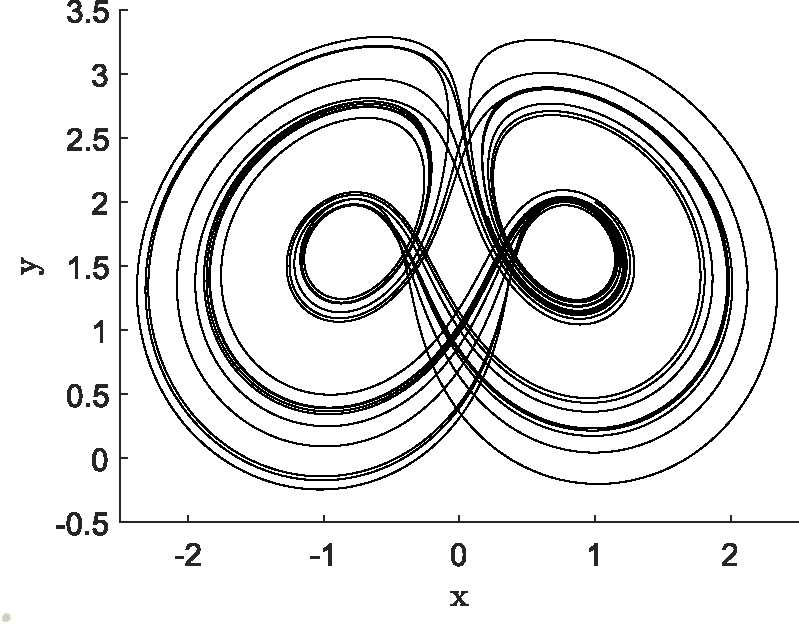
\includegraphics[scale=0.28]{files/int_adams_xy.pdf}
\end{subfigure}
\begin{subfigure}[ht]{0.3\textwidth}
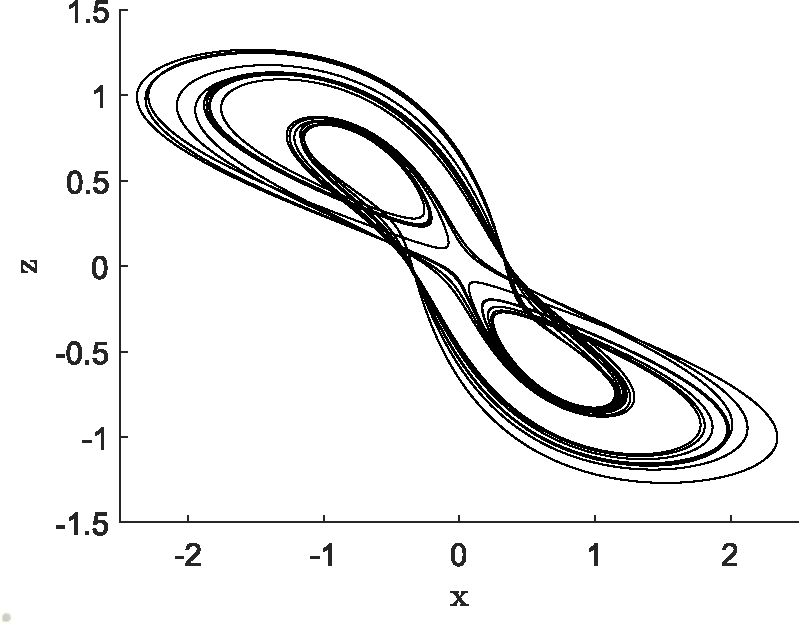
\includegraphics[scale=0.28]{files/int_adams_xz.pdf}
\end{subfigure}
\begin{subfigure}[ht]{0.3\textwidth}
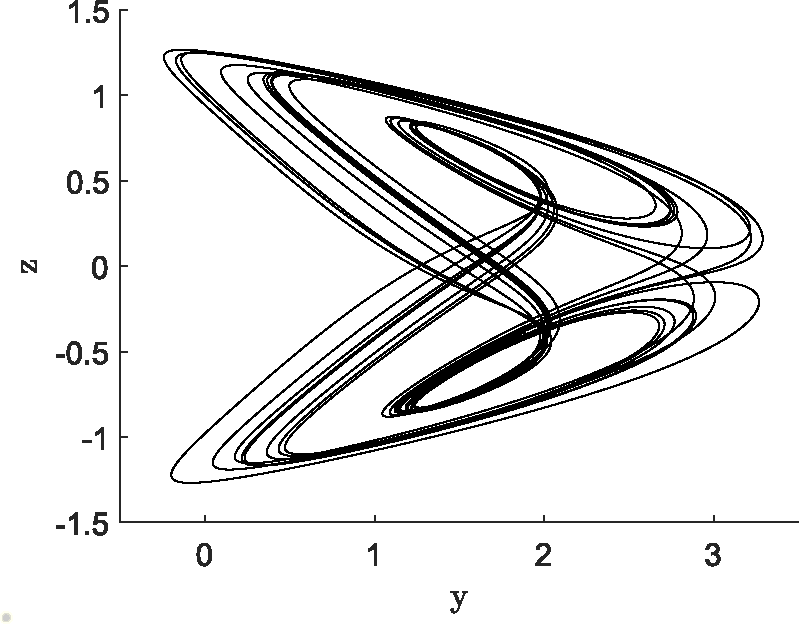
\includegraphics[scale=0.28]{files/int_adams_yz.pdf}
\end{subfigure}
\caption{Simulation Results: phase portraits.}
\label{fig:financeValidation}
\end{figure}
Now, in order to make a further validation of the presented algorithm, we will illustrate an example with a fractional initial value problem.
\begin{exmp}\label{ex:adam}
Solve the following the fractional initial value problem using ABM, with $y(0) = 1$ and $y'(0) = 0$.
\begin{equation}
    \mathcal{D}_c^{1.25}y(t)=-y(t)
\end{equation}
\end{exmp}
Carrying out some analytic operations, the exact solution is given by
\begin{equation}
    y(t) = E_{1.25,\,1}(-t^{1.25})=\sum_{k=0}^{\infty}\dfrac{(-1)^kt^{1.25k}}{\Gamma(1.25k +1)} 
\end{equation}
The ABM method was executed with different time-steps $h$ in order to show how the exact solution is better approximated for smaller values of $h$. The plot for the results are shown in figure \ref{fig:exAdams}; on the other hand, table \ref{tab:exAdams} shows the numeric approximation in certain values of $t$. Note that all approximations stabilize around the same value.
\begin{table}[H]
\centering
\begin{tabular}{cccccc}
\hline
\textbf{Time}    & \boldmath{$h=0.5$} & \boldmath{$h=0.25$} & \boldmath{$h=0.1$} & \boldmath{$h=0.01$} & \textbf{Exact}   \\ \hline
\boldmath{$t=0$} & 1                  & 1                   & 1                  & 1                   & 1       \\
\boldmath{$t=1$} & 0.0144             & 0.2147              & 0.3096             & 0.3601              & 0.3655  \\
\boldmath{$t=2$} & -0.1288            & -0.0527             & -0.0174            & 0.0016              & 0.0036  \\
\boldmath{$t=3$} & -0.1182            & -0.1065             & -0.1018            & -0.0992             & -0.0989 \\
\boldmath{$t=4$} & -0.0773            & -0.0854             & -0.0899     & -0.0923             & -0.0926 \\
\boldmath{$t=5$} & -0.0454            & -0.0547             & -0.0596            & -0.0622             & -0.0625 \\
\boldmath{$t=6$} & -0.0274            & -0.0335             & -0.0366            & -0.0383             & -0.0385 \\
\boldmath{$t=7$} & -0.0188            & -0.0221             & -0.0236            & -0.0245             & -0.0246 \\ \hline
\end{tabular}
\caption{Numerical results using ABM algorithm for different step sizes.}
\label{tab:exAdams}
\end{table}
\begin{figure}[H]
    \centering
    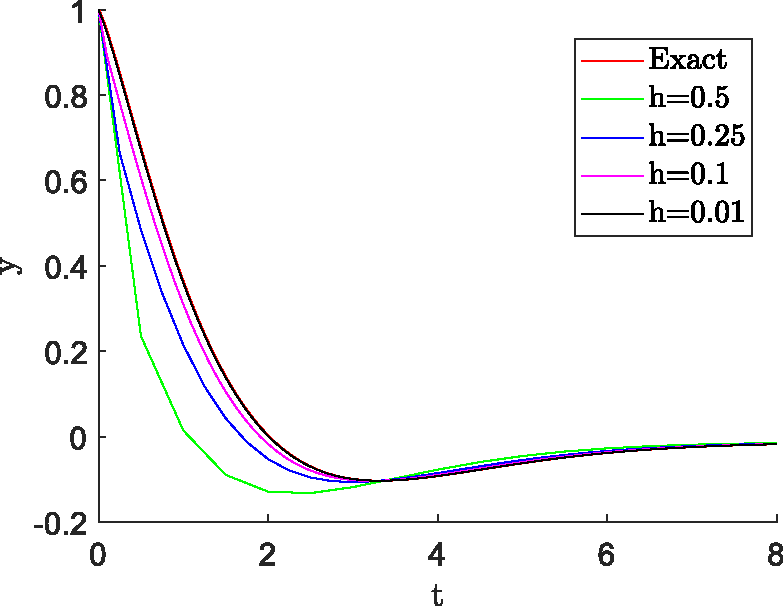
\includegraphics[scale=0.5]{files/ejemplo_adam.pdf}
    \caption{Results for different step-sizes using ABM predictor-corrector.}
    \label{fig:exAdams}
\end{figure}

\begin{exmp}
Chua Fractional System
\end{exmp}

The Chua system is given by:
\begin{equation}
    \begin{cases}
        \mathcal{D}_c^\alpha x(t) = a\left[x_2(t)-x_1(t)-f(x_1)\right]&\\
        \mathcal{D}_c^\alpha y(t) = x_1(t)-x_2(t)+x_3(t)&\\
        \mathcal{D}_c^\alpha z(t) = -bx_2(t)-cx_3(t)
    \end{cases}
\end{equation}
In our case, in order to compare with the results obtained in \cite{yang2018generation}, $\alpha=0.95$, $a=10.725$, $b=10.593$, $c = 0.268$, $m0 = -1.1726$, $m1 = -0.7872$ and
\begin{equation*}
    f(x_1)=m_1x_1(t)+\dfrac{1}{2}(m_0+m_1)\left(|x_1(t)+1|-|x_1(t)-1|\right)
\end{equation*}
with initial conditions $(x_0,\,y_0,\,z_0)=(-0.2,\, -0.1,\, 0.1)$, obtaining the following results:

\begin{figure}[H]
\centering
\begin{subfigure}[ht]{0.45\textwidth}
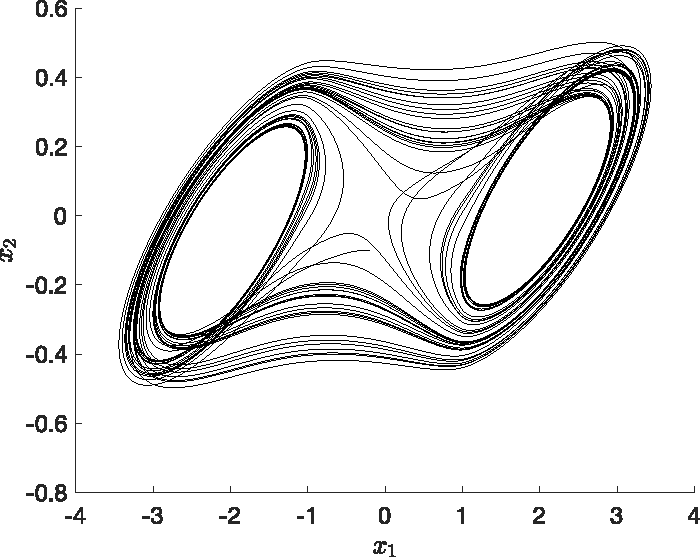
\includegraphics[scale=0.4]{files/ChuaX2vsX1_q0-95.pdf}
\end{subfigure}
\begin{subfigure}[ht]{0.45\textwidth}
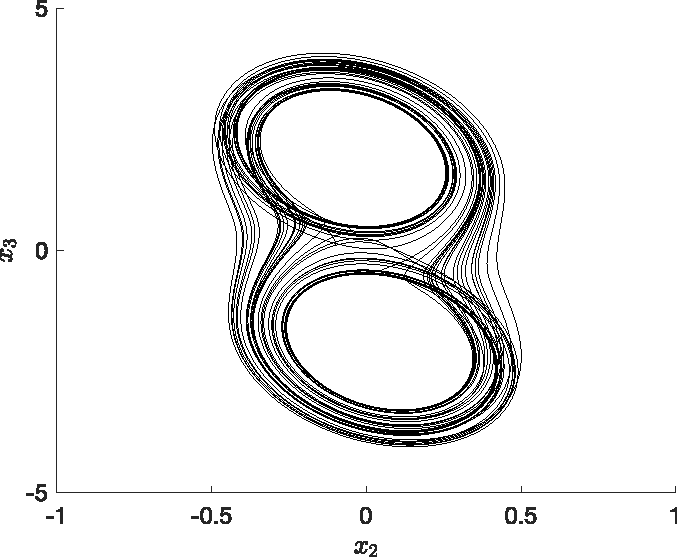
\includegraphics[scale=0.4]{files/ChuaX2vsX3_q0-95.pdf}
\end{subfigure}
\caption{Fractional Chua system: phase planes.}
\label{fig:Exchua}
\end{figure}

Which can be directly compared with figure 3 of Yang \textit{et al.} in \cite{yang2018generation}, obtaining the same results.

\begin{exmp}\label{ex:adam_disp}
ABM with explicit time
\end{exmp}

Solve the following initial value problem using ABM method, notice that in this problem the time is explicit in the differential equation.

\begin{equation} 
\mathcal{D}_{c}^{\alpha} y(t)= \frac{40320}{\Gamma(9-\alpha)} t^{8-\alpha}-3 \frac{\Gamma(5+\alpha / 2)}{\Gamma(5-\alpha / 2)} t^{4-\alpha / 2}+\frac{9}{4} \Gamma(\alpha+1)+\left(\frac{3}{2} t^{\alpha / 2}-t^{4}\right)^{3}-[y(t)]^{3 / 2} 
\end{equation}

Carrying out some analytic operations, with $\alpha=1.25 , y(0) = 1$ and $y'(0)=0$ the exact solution is given by:

\begin{equation}
    y(t) = t^{8}-3 t^{4+\alpha /2}+\frac{9}{4} t^{\alpha}
\end{equation}

The ABM, was performed with a step-size of $h=0.004$. In the figure \ref{fig:adam_disp}, it is shown a comparison between the exact solution and ABM, it can been that the numerical solution overlaps the exact solution, during the most of the simulation. It is important to remark that is a small time of simulation.

\begin{figure}[H]
    \centering
    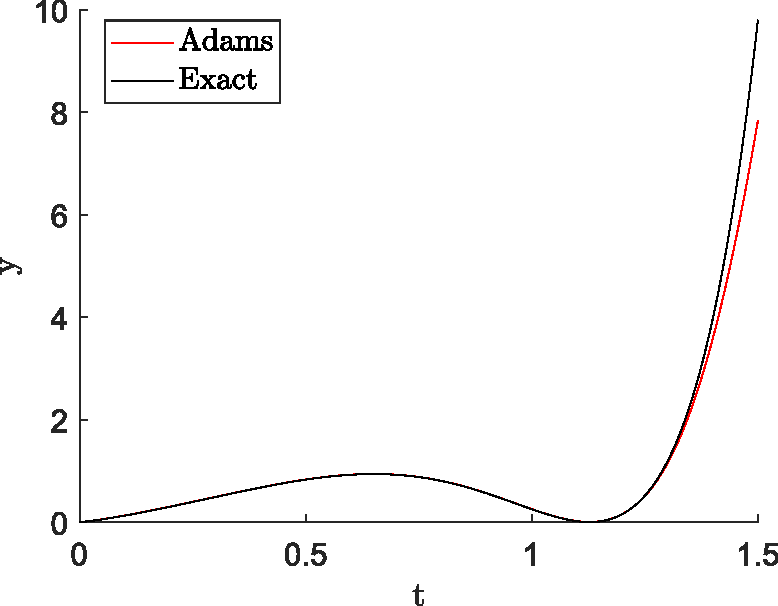
\includegraphics[scale=0.5]{files/adams_exact_xt_with_dispersion.pdf}
    \caption{ABM for fractional differential equations with explicit time, $T=1.5$.}
    \label{fig:adam_disp}
\end{figure}

In the figure \ref{fig:adam_disp2}, the time of the simulation was doubled, this clearly shows that when the time is explicit the behaviour of the numerical method diverges for big time of simulation, also is important to say that a comparison to the previous figure it is not valid to always assume that the performance of the system is going to continue approximating in a good way to the exact solution.

\begin{figure}[H]
    \centering
    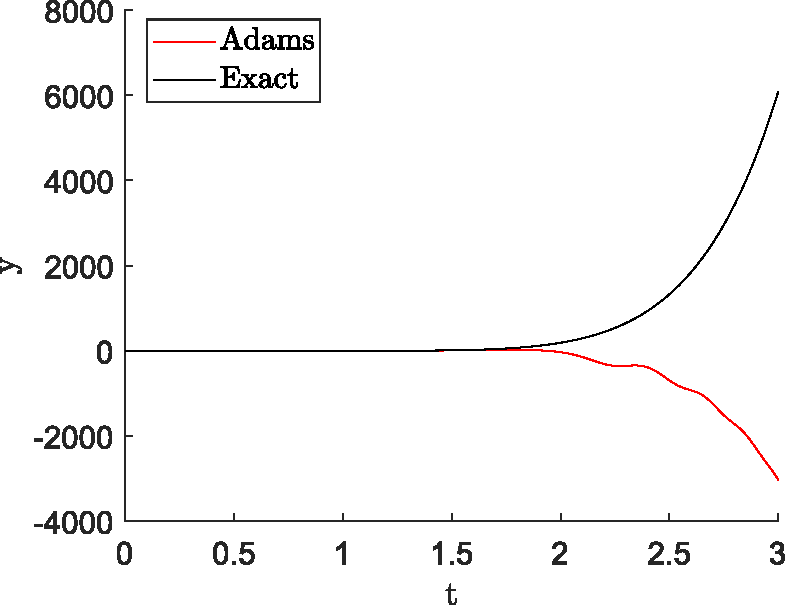
\includegraphics[scale=0.5]{files/adams_dispersion_2.pdf}
    \caption{ABM for fractional differential equations with explicit time, $T=3$.}
    \label{fig:adam_disp2}
\end{figure}

